\documentclass[tikz,border=2pt]{standalone}
\usepackage{amsmath,amssymb}
\usepackage{tikz}
\usetikzlibrary{arrows.meta}

\begin{document}
% A point P lies in the plane exactly when the vector from the fixed point P0 to P is
% perpendicular to the normal n: n . (P - P0) = 0.
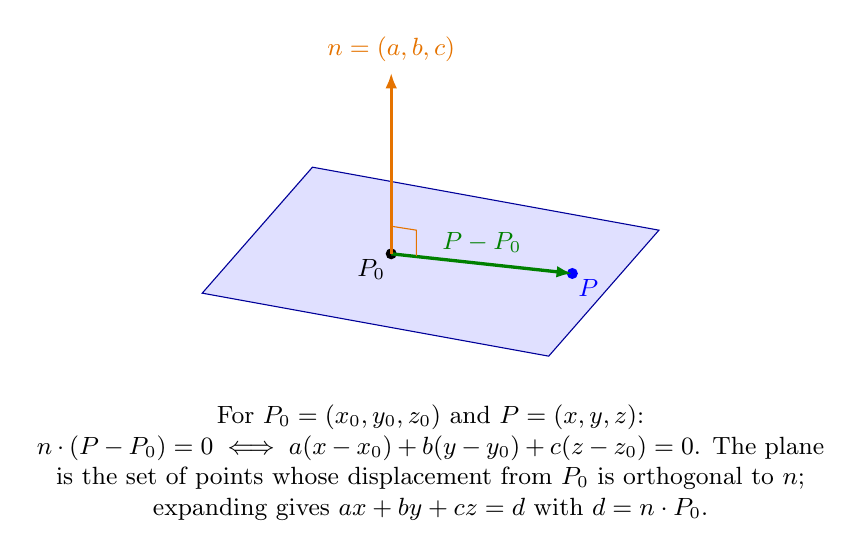
\begin{tikzpicture}[every node/.style={font=\small}, >={Latex[length=2mm]}]
	\fill[blue!12] (-1.8,0.2) -- (2.6,-0.6) -- (4.0,1.0) -- (-0.4,1.8) -- cycle;
	\draw[blue!60!black] (-1.8,0.2) -- (2.6,-0.6) -- (4.0,1.0) -- (-0.4,1.8) -- cycle;
	\coordinate (P0) at (0.6,0.7);
	\coordinate (P) at (2.9,0.45);
	\fill (P0) circle (2pt) node[below left, inner sep=2pt] {$P_0$};
	\fill[blue] (P) circle (2pt) node[below right, inner sep=2pt] {$P$};
	\draw[->, green!50!black, very thick] (P0) -- (P) node[midway, above, font=\small] {$P-P_0$};
	\draw[->, orange!90!black, very thick] (P0) -- (0.6,3.0) node[above] {$n=(a,b,c)$};
	\draw[orange!90!black] (0.6,1.05) -- (0.92,1.0) -- (0.92,0.67);
	\node[anchor=north, align=flush center, text width=10cm] at (1.1,-1.1) {For $P_0=(x_0,y_0,z_0)$ and $P=(x,y,z)$: $n\cdot(P-P_0)=0\iff a(x-x_0)+b(y-y_0)+c(z-z_0)=0$. The plane is the set of points whose displacement from $P_0$ is orthogonal to $n$; expanding gives $ax+by+cz=d$ with $d=n\cdot P_0$.};
\end{tikzpicture}
\end{document}
